%%%%%%%%%%%%%%%%%%%%%%%%%%%%%% -*- Mode: Latex -*- %%%%%%%%%%%%%%%%%%%%%%%%%%%%
%% proposal.tex -- 
%% Author          : Robert Brewer
%% Created On      : Tue Jan 10 11:53:15 1995
%% Last Modified By: Robert Brewer
%% Last Modified On: Mon Jan 31 16:48:09 2000
%% Status          : Unknown
%% RCS: $Id: proposal.tex,v 1.3 1999/02/02 04:17:26 rbrewer Exp $
%%%%%%%%%%%%%%%%%%%%%%%%%%%%%%%%%%%%%%%%%%%%%%%%%%%%%%%%%%%%%%%%%%%%%%%%%%%%%%%
%%   Copyright (C) 1998 Robert Brewer
%%%%%%%%%%%%%%%%%%%%%%%%%%%%%%%%%%%%%%%%%%%%%%%%%%%%%%%%%%%%%%%%%%%%%%%%%%%%%%%
%% 
%% For building official version w/o titlepage or abstract
\documentclass [11pt] {article}

%% New LaTeX2e graphics support
\usepackage[final]{graphicx}
%% Support for decent URL output
\usepackage{url}
%% Switch to Times Postscript font
\usepackage{times}

%% Make the margins sane, must be in preamble to work properly
\setlength{\oddsidemargin}{0in}
\setlength{\textwidth}{6.5in}
\setlength{\textheight}{8.6in}
\setlength{\topmargin}{0in}
\setlength{\headheight}{0in}
\setlength{\headsep}{0in}
\setlength{\topskip}{1pt}
\setlength{\footskip}{0.75in}

\title{Aspect Technology Fund Grant Proposal:\\Adaptive Spam Detection and
Removal Tool}
\author{Robert S. Brewer\\Collaborative Software Development Lab\\University of
Hawaii at Manoa}

\date{February 1, 2000}

\begin{document}

%% For building CSDL internal version with titlepage and abstract
%\maketitle

%\begin{abstract}
%  Spam tool abstract to be written...
%\end{abstract}

%%%%%%%%%%%%%%%%%%%%%%%%%%%%%% -*- Mode: Latex -*- %%%%%%%%%%%%%%%%%%%%%%%%%%%%
%% project-description.tex -- 
%% Author          : Robert Brewer
%% Created On      : Wed Jan 27 16:28:11 1999
%% Last Modified By: Carleton Moore
%% Last Modified On: Mon Feb  1 12:31:41 1999
%% RCS: $Id$
%%%%%%%%%%%%%%%%%%%%%%%%%%%%%%%%%%%%%%%%%%%%%%%%%%%%%%%%%%%%%%%%%%%%%%%%%%%%%%%
%%   Copyright (C) 1999 Robert Brewer
%%%%%%%%%%%%%%%%%%%%%%%%%%%%%%%%%%%%%%%%%%%%%%%%%%%%%%%%%%%%%%%%%%%%%%%%%%%%%%%
%% 

\section{Project Description}
%No more than 1000 words

\subsection{Introduction}
% 82 words

The people of Hawaii are focusing new effort and emphasis on support for
small business.  The initial development of a small business depends upon
many factors, but one of the most important is a high quality business
plan: a roadmap that describes what the business is, why it can be
successful, and how it will be organized and operate over time.  The best
business plans are living documents that evolve and change to reflect the
growth and maturation of the organization.

\subsection{The Problem With Current Business Plan Development}
%What problem are you solving?
% 166 words

Many entrepreneurs do not develop business plans before they start their
business or the business plan they develop is not a good one.  There are
many barriers to developing a good business plan; there is little or no
feedback on the business plan, there are few, if any, sources of checklists
for developing good business plans, and there are very few repositories
where entrepreneurs can learn from examples of a variety of business plans.

Entrepreneurs rarely get their business plans reviewed before they start to
shop it around for venture capital.  This is too late in the development
cycle.  First impressions are very difficult to overcome.  An entrepreneur
with a poor business plan has a low chance of getting their business
funded.

There are very few places for entrepreneurs to find localized advice on
developing business plans.  The many books and web sites on business plan
writing are intended for a global or national audience.  The solutions are
not tailored to Hawaii's unique business environment.


\subsection{Applying Software Engineering Principles to Business Plan Development}
%What is the solution to the problem?
% 265 words

I propose that many of these problems in the development of high quality
business plans can be solved by applying principles from software
engineering.  The three software engineering principles I propose to apply
are distributed review, defect collection and management, and patterns.  By
conducting reviews of early drafts of a business plan we can ensure that
the final version shown to the venture capitalists is of high quality and
provides a positive first impression.  If we collect the defects found in
the early drafts of the business plan we can develop checklists of common
problems encountered in business plan development.  Entrepreneurs can use
these checklists to avoid common problems.  By analyzing the defects
collected and the actual business plans we can develop patterns for
successful business plans.


Project LEAP and the Leap Toolkit support distributed review, defect
collection and management and patterns.  You can find more information
about project LEAP and the Leap Toolkit at the following web site.
\url{<http://csdl.ics.hawaii.edu/Research/LEAP/LEAP.html>} The Leap Toolkit
is a general purpose mechanism for technical skill acquisition and
improvement. Currently, it is in use to support software development and
technical writing. With this grant, I will adapt the Leap Toolkit to
support the development and improvement of business plans in the State of
Hawaii. Entrepreneurs will use Leap to obtain useful reviews of their
business plans, to access and contribute helpful checklists that detect
common problems in local business plans, and to learn from and generate
new patterns that represent common features of and approaches to successful
Hawaii business plans.

\subsubsection{Usage Scenario}
%How will it actually work?
% 184 words 

Entrepreneur Cam wants to start a new business in Hawaii.  He needs to
write his business plan so he checks the Leap Business Plan Web Site to get
some good patterns for successful business plans.  Cam finds three patterns
that he wants to use.  Before he starts writing his plan he down-loads a
couple of checklists describing the most common errors made by new
entrepreneurs (see figure \ref{fig:checklist}).  By studying these
checklists Cam successfully avoids these pit-falls and saves many
frustrating hours in development.  After writing his draft plan Cam submits
the plan to the Leap Web site for review.  Volunteer reviewers review Cam's
plan and note several defects with the plan.  These defects are recorded in
Leap so Cam can easily track them and the defects are added to the Leap
Business Plan Web Site defect repository for later analysis.  Cam fixes the
few defects with his plan, gets his venture capital and starts a very
successful small business.  After setting up his successful business, Cam
contributes new checklists and patterns to the Leap Business Plan Web Site.

\begin{figure}[htb]
  \centering
  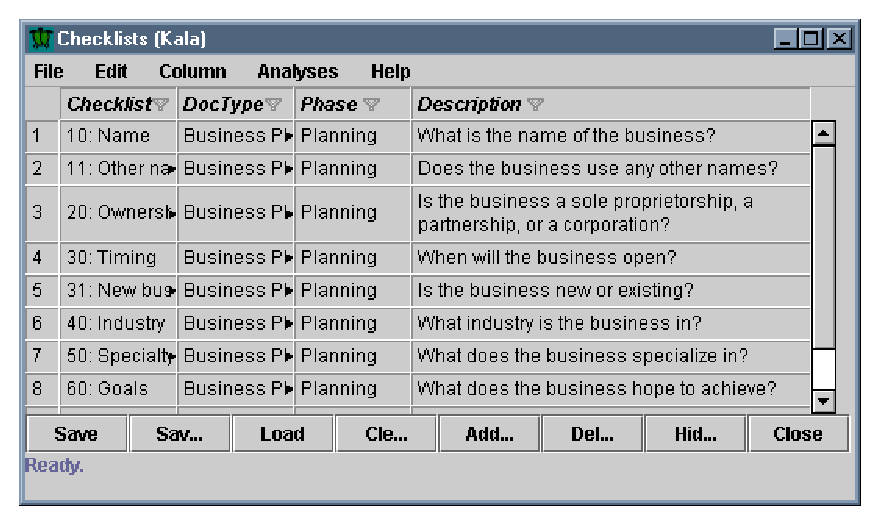
\includegraphics{checklist.eps}
  \caption{Mockup of Business Plan checklist in LEAP}
  \label{fig:checklist}
\end{figure}


%\subsection{Business Plan}
%How will this make money?
%What is the revenue potential?
% words

\subsection{Competing Technologies}
%Why is your solution unique?
% 175 words

Searching the web on Yahoo! I found many sites devoted to small business
development and business plan development.  Here is a sample:
\begin{itemize}

\item {Yahoo! Small Business
    \url{http://smallbusiness.yahoo.com}  provides links to resources for
    small businesses.  There are some links to books and suggestions for
    writing business plans, but no checklists or review services.}

\item {American Express Small Business Services
    \url{http://www6.americanexpress.com/smallbusiness/resources/starting/biz_plan} 
    gives outlines for business plans and good reasons for having a plan.
    There are some very general patterns for good business plans. However,
    this site does not have any specific information on local Hawaii conditions.}
  
\item {BizPlanIt.Com \url{http://www.bisplanit.com} looks like a company
    that write your business plan after talking to you.  There are no public
    checklists or patterns.  This might be a good model for a future
    commercialization of the Leap Business Plan Web Site.}
  
\end{itemize}

None of these sites focus on any local issues or provide facilities for
reviewing existing drafts of plans.

\subsection{Risks Involved}
% 123 words

%Risks in development
%Risk abatement plan

There are several risks to this project. First, can we transfer the software
engineering principles to business plan development?  Second, there are privacy
issues involved with business plans that must be addressed in the system.

This grant will provide an opportunity to address the first risk, by
providing the ability to develop a small prototype version and evaluate its
impact.

The second issue of privacy also exists in software development and we can
apply technology we are developing there to this domain.  One solution is
to provide a tool to make the Leap data anonymous.  The checklists and
patterns will not refer to any developer.  We will develop mechanisms for
submitting the business plans for review that will ensure the developer's
privacy.


%\subsection{Technical Infrastructure}
%% 49 words

%%development infrastructure
%University of Hawaii equipment editor, Java.  Business plan anonymizer to
%remove the sensitive portions of the plan or another mechanism for brining
%in your plan to the centers and submitting them for review.

%%customer infrastructure (requirements)

%Java, fast machine, Internet connection for web browsing, submission of
%business plan.


%\subsection{Future Potential}
%%Next steps/scale up
%% 51 words

%Hawaii Small Business Development Centers future partners?  provide
%reviewers, users, training in the tools,  analysis support etc.  Either go
%commercial like BPlans or BisPlanIt.com or go non profit to support
%Hawaii's economy.

%Local repository for great business plan suggestions.  Increase in the
%local economy.  Higher quality businesses. 

\subsection{Project Plan}
%What is the timeline for the project?
%What milestones are there along the way to completion?
%What are the deliverables?
% 33 words
\begin{table}[htb]
  \begin{tabular}{ll}
    Mile Stone & Date \\ \hline
    Leap ToolKit Available& Now \\
    Tool to make Leap data anonymous& Summer, 1999 \\
    Web Based Repository of Leap Data& Spring, 2000 \\
    Pilot Leap Business Plan development site& Summer, 2000 \\ \hline
  \end{tabular}
\end{table}
      

\subsubsection{Deliverables}
% 42 words
I plan on delivering the following: an Open Source distribution of Leap
Toolkit, a Web based Leap data repository, a tool to make Leap data
anonymous, a pilot Leap Business Plan development site,  and a technical
report on our lessons learned.


%%%%%%%%%%%%%%%%%%%%%%%%%%%%%% -*- Mode: Latex -*- %%%%%%%%%%%%%%%%%%%%%%%%%%%%
%% budget.tex -- 
%% Author          : Robert Brewer
%% Created On      : Wed Jan 27 14:53:13 1999
%% Last Modified By: Carleton Moore
%% Last Modified On: Sat Jan 30 14:49:44 1999
%% RCS: $Id$
%%%%%%%%%%%%%%%%%%%%%%%%%%%%%%%%%%%%%%%%%%%%%%%%%%%%%%%%%%%%%%%%%%%%%%%%%%%%%%%
%%   Copyright (C) 1999 Robert Brewer
%%%%%%%%%%%%%%%%%%%%%%%%%%%%%%%%%%%%%%%%%%%%%%%%%%%%%%%%%%%%%%%%%%%%%%%%%%%%%%%
%% 

\section{Project Budget}
%No more than 1 page

The project budget consists of: A computer to serve as the web server for
the Leap Business Plan Developer's Web site, printing, graphics and postage
costs for developing and distributing training manuals and advertising, and
travel expenses for contacting business experts.

There may be small variations in the price of the equipment when the order
is actually placed due to bundling offers from manufactures, etc. Microsoft
Office 98 can be obtained from the UH Bookstore.

\vspace{1 in}

%\setlength{\topmargin}{0in}
%\setlength{\headheight}{0in}
%\setlength{\headsep}{0in}
%\setlength{\topskip}{1pt}

\begin{table}[htb]
  \begin{center}
    \begin{tabular}{lcr@{.}l}
      Item & \multicolumn{2}{c}{Budget}\\ \hline
      \large {\bf Pentium II Computer} &  & \$ 3846 & 00 \\
      Intel 450MHz Pentium II Processor w/ 512K cache & &
      \multicolumn{2}{c}{} \\
      256MB 100MHz SDRAM & & \multicolumn{2}{c}{} \\
      VX1100 21inch color monitor& &\multicolumn{2}{c}{} \\
      16MB AGP Graphics Accelerator& &\multicolumn{2}{c}{} \\
      16.8GB 5400RPM Ultra ATA hard drive& &\multicolumn{2}{c}{} \\
      3.5inch 1.44MB diskette drive & &\multicolumn{2}{c}{} \\
      IOMEGA internal zip drive & &\multicolumn{2}{c}{} \\
      DVD III-ROM Drive& &\multicolumn{2}{c}{} \\
      Philips Recordable/ReWriteable CD-ROM& &\multicolumn{2}{c}{} \\
      Intel EtherExpress Pro/100+ & & \multicolumn{2}{c}{} \\
      Telepath 56K Modem & & \multicolumn{2}{c}{} \\
      MS Office 97, Professional & & \multicolumn{2}{c}{} \\
      Windows NT Workstation & &\multicolumn{2}{c}{} \\
      104+ Keyboard  & & \multicolumn{2}{c}{} \\

      Printing \& Graphics& & \$ 500 & 00 \\
      Postage & & \$ 100 & 00 \\
      Travel \& Parking & & \$ 500 & 00 \\
      \hline
      {\bf Total}&& \$ 4946 & 00 \\
    \end{tabular}
  \end{center}
\end{table}




%%%%%%%%%%%%%%%%%%%%%%%%%%%%%% -*- Mode: Latex -*- %%%%%%%%%%%%%%%%%%%%%%%%%%%%
%% essay.tex -- 
%% Author          : Robert Brewer
%% Created On      : Wed Jan 27 17:17:21 1999
%% Last Modified By: Robert Brewer
%% Last Modified On: Mon Jan 31 12:29:00 2000
%% RCS: $Id: essay.tex,v 1.1 2000/01/31 22:12:58 rbrewer Exp rbrewer $
%%%%%%%%%%%%%%%%%%%%%%%%%%%%%%%%%%%%%%%%%%%%%%%%%%%%%%%%%%%%%%%%%%%%%%%%%%%%%%%
%%   Copyright (C) 1999 Robert Brewer
%%%%%%%%%%%%%%%%%%%%%%%%%%%%%%%%%%%%%%%%%%%%%%%%%%%%%%%%%%%%%%%%%%%%%%%%%%%%%%%
%% 

\section{Essay Question}
%No more than 700 words, currently exactly 700 words (not counting heading and quote)

\begin{quote}
  {\em As an Aspect Technology Fund grant recipient, how would you contribute
    to the field of technology and promote the spirit of entrepreneurship?}
\end{quote}

As a grant recipient I will be helping the growth of high-tech industry here in
Hawaii. In the last few months it seems like all politicians and the media can
do is talk about high-tech and what it can do for Hawaii. In his 2000 ``State
of the State'' address the governor highlighted technology as an area where the
state needs to continue to expand. But it takes more than words to build a
business. It takes people actually willing to take risks and make a commitment
to hard work.

I have already been involved in one successful high-tech startup here in
Hawaii: LavaNet. I left the MS program in ICS to help start LavaNet in 1994.
Through a lot of hard work, in 1997 LavaNet had grown to employ 23 people and
serve 6,500 customers. At that time I decided to come back to UH to finish my
degree.

One of the very real problems with the high-tech industry here in Hawaii is the
migration of talented people to the mainland. The booming Silicon Valley
economy makes it difficult to convince technical people to stay in Hawaii. My
experiences at LavaNet I have enabled me to evangelize the concept of
entrepreneurship with first hand experience. Many students here at UH have not
seriously considered being part of a startup company here in Hawaii as a career
path which is unfortunate. This grant would form the foundation of a software
business based here in Hawaii.  Beyond the initial implementation, developers
will be needed to enhance existing spam tests and add new ones. The server
product will require a skilled technical support staff in order to help ISPs
install the software. There is a lot of potential for this kind of enterprise
because for information technology, Hawaii's geographical isolation is
irrelevant. Also, information technology has virtually no environmental impact
compared to other industries, which makes it sustainable.

I'm also pleased to hear that there is more venture capital available for
high-technology now than ever before. Most of the credit for this must go to
the incredible success of the Digital Island IPO. In my opinion the best way to
promote the spirit of entrepreneurship is to lead by example. Each successful
technology company further demonstrates that it is possible (and profitable) to
start up in Hawaii which encourages others to take the entrepreneurial leap.
And those that payoff big for their investors will provide the seed funds for
more companies (as Digital Island has done).

In conclusion, I have the experience and the ability to take an idea and turn
it into a company. Every high tech company that starts up and succeeds in
Hawaii provides another beacon for future entrepreneurs.

% LocalWords:  http opensource LocalWords tex www org Exp


\end{document}

%% Woo woo! $5000 here I come! :)
